\let\negmedspace\undefined
\let\negthickspace\undefined
\documentclass[journal]{IEEEtran}
\usepackage[a5paper, margin=10mm, onecolumn]{geometry}
%\usepackage{lmodern} % Ensure lmodern is loaded for pdflatex
\usepackage{tfrupee} % Include tfrupee package

\setlength{\headheight}{1cm} % Set the height of the header box
\setlength{\headsep}{0mm}     % Set the distance between the header box and the top of the text

\usepackage{gvv-book}
\usepackage{gvv}
\usepackage{cite}
\usepackage{amsmath,amssymb,amsfonts,amsthm}
\usepackage{algorithmic}
\usepackage{graphicx}
\usepackage{textcomp}
\usepackage{xcolor}
\usepackage{txfonts}
\usepackage{listings}
\usepackage{enumitem}
\usepackage{mathtools}
\usepackage{gensymb}
\usepackage{comment}
\usepackage[breaklinks=true]{hyperref}
\usepackage{tkz-euclide} 
\usepackage{listings}
% \usepackage{gvv}                                        
\def\inputGnumericTable{}                                 
\usepackage[latin1]{inputenc}                                
\usepackage{color}                                            
\usepackage{array}                                            
\usepackage{longtable}                                       
\usepackage{calc}                                             
\usepackage{multirow}                                         
\usepackage{hhline}                                           
\usepackage{ifthen}                                           
\usepackage{lscape}
\begin{document}

\bibliographystyle{IEEEtran}
\vspace{3cm}

\title{}
\author{EE24BTECH11053 - S A Aravind Eswar
}
% \maketitle
% \newpage
% \bigskip
{\let\newpage\relax\maketitle}

\renewcommand{\thefigure}{\theenumi}
\renewcommand{\thetable}{\theenumi}
\setlength{\intextsep}{10pt} % Space between text and floats


\numberwithin{equation}{enumi}
\numberwithin{figure}{enumi}
\renewcommand{\thetable}{\theenumi}

\textbf{Question:} Find the value of $x$ if the distance between points $\vec{A}\myvec{0\\0}$, and $\vec{B}\myvec{$x$\\4}$ is 5 units.\\

\solution
\begin{table}[h]
	\centering
	\begin{tabular}{|m{5em} | m{5em} | m{10em} |}
	\hline
	\textbf{Symbol} & \textbf{Value} &\textbf{Description}\\
	\hline
		\textbf{A} & $\myvec{0\\0}$ & Point \textbf{A}\\
	\hline
		\textbf{B} & $\myvec{x\\-4}$ & Point \textbf{B}\\
	\hline
		$d$          & 5              & Distance between points \textbf{A} and \textbf{B}\\
	\hline
\end{tabular}

	\caption{Given Values}
	\label{tab:1}
\end{table}

Given,

\begin{align}\norm{{AB}} = d\\\norm{{AB}}^2 = d^2\\AB^tAB = d^2\\\brak{\myvec{1 & 0\\0 & 0}\brak{\vec{B}-\vec{A}}+\myvec{0 & 0\\0 & 1}\brak{\vec{B}-\vec{A}}}^\top\brak{\myvec{1 & 0\\0 & 0}\brak{\vec{B}-\vec{A}}+\myvec{0 & 0\\0 & 1}\brak{\vec{B}-\vec{A}}} = d^2\\\brak{\vec{B}-\vec{A}}^\top\myvec{1 & 0\\0 & 0}\brak{\vec{B}-\vec{A}} + \brak{\vec{B}-\vec{A}}^\top\myvec{0 & 0\\0 & 1}\brak{\vec{B}-\vec{A}} = d^2\\\brak{\vec{B}-\vec{A}}^\top \vec{e_1} \vec{e_1}^\top\brak{\vec{B}-\vec{A}} + \brak{\vec{B}-\vec{A}}^\top\vec{e_2}\vec{e_2}^\top\brak{\vec{B}-\vec{A}} = d^2\\\norm{\vec{e_1}^\top\brak{\vec{B}-\vec{A}}}^2 + \norm{\vec{e_2}^\top\brak{\vec{B}-\vec{A}}}^2 = d^2\\\vec{e_1}^\top\vec{B} = \vec{e_1}^\top\vec{A} + \sqrt{d^2 - \brak{\vec{e_2}^\top\brak{\vec{B}-\vec{A}}}}\end{align}
Solving,\\
	\begin{align}x = 3  \text{ (or) }  x = -3\end{align}

\begin{figure}[h]
    \centering
    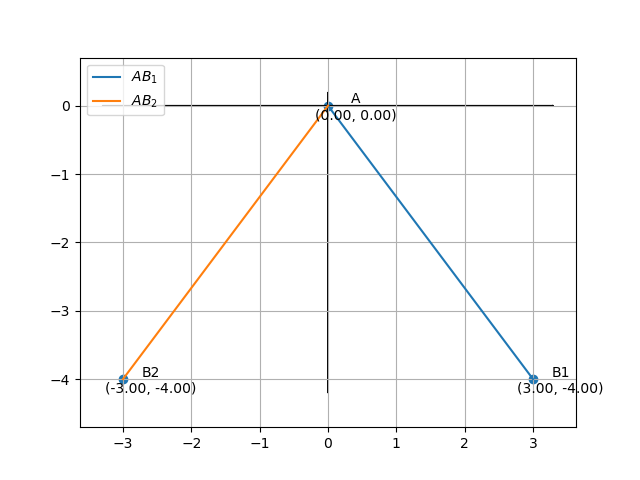
\includegraphics[width=\columnwidth]{figs/fig0.png}
    \caption{Points \textbf{A},\textbf{B},\textbf{C} and \textbf{D}}
 \end{figure}

\end{document}  

